\documentclass[tikz, convert={outext=.png}]{standalone}

% use xelatex
\usepackage{fontspec}
\usepackage{pgffor}

\setmainfont{Ubuntu Mono}

\begin{document}

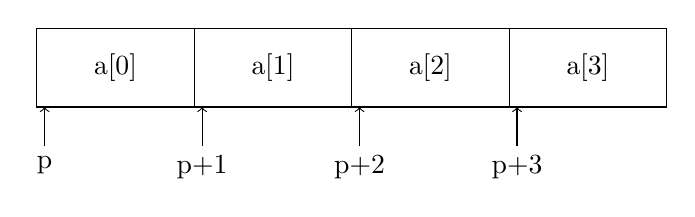
\begin{tikzpicture}
  \foreach \i in {0, 1, 2, 3} {
    \node[rectangle, draw, minimum width = 2cm, minimum height = 1cm] (r\i) at (\i * 2, 0) {};
    \node at (r\i.center) {a[\i]};
    \draw[->] (\i * 2 - 0.9, -1) -- (\i * 2 - 0.9, -0.5);
  }
  \node[below] at (-0.9, -1) {p};
  \foreach \i in {1, 2, 3} {
    \node[below] at (\i * 2 - 0.9, -1) {p+\i};
  }
\end{tikzpicture}

\end{document}